\chapter{Entwicklung und Testing}
\label{chap:testing}

\section{Entwicklung des Frontends}
Hier wurde der Node Package Manager (\emph{npm}) verwendet, um die Dependencies zu beziehen. Mit Webpack wurde das Javascript und die vue-Template Dateien in eine Javascript-Datei kompiliert. Webpack bringt mit dem Befehl \emph{npm run dev} auch gleich einen kleinen Webserver mit, welcher den Vorteil bringt, dass man nicht nach jeder Änderung den Code neu kompilieren muss, sonder dieser laufend im Browser aktualisiert (injected) wird.

\section{Entwicklung des Backends}
Für die Entwicklung der API wurde, wie bereits erwähnt, Laravel eingesetzt. Für den lokalen Betrieb wird eine Virtuelle Maschine empfohlen. Hier wurde Vagrant mit einem Homestead Container verwendet. Als Datenbank kam das mit dem Homestead mitgelieferte mySQL zum Einsatz.

Die Virtuelle Maschine kann durch den lokal eingerichteten Pfad \url{http://presentator3000.app/api/} angesteuert werden.

Um das Zusammenspiel der API mit dem Frontend zu testen, wurde auf einem Webserver eine Stage aufgesetzt. Die Zugänge lauten wie folgt:

\begin{itemize}
	\item \textbf{Frontend:} \url{http://3000.uahnn.com/}
	\item \textbf{Backend:} \url{http://presentator3000.uahnn.com/api/}
\end{itemize}

Zudem wurden bei der API 2 Routen angelegt, eine für die URL direkt und eine für \emph{/api} mit Testcontent, um die Funktionalität einfach zu überprüfen (läuft das System noch).

Um die Datenbank zu testen, wurden mit Hilfe von Seedern Demo-Daten abgefüllt. Die Datenbank-Tabellen wurde nicht direkt mit SQL Queries angelegt, sondern durch Migrations (in Laravel). Dies sind PHP-Container, welche durch Methoden die jeweiligen Tabellen und Felder anlegen. Dies ermöglichte eine laufende Anpassung des Datenbank-Modells. Bei jeder Anpassung konnten so die Demodaten durch die Seeder erneut erzeugt werden. Somit hat man zu jeder Zeit passende Demo-Daten. 

\section{Testing der API}
Um die Entwicklung von API und Frontend unabhängig von einander voranzutreiben, mussten die API-Calls separat getestet werden. Hier wurde das Tool \emph{Postman} verwendet. Es handelt sich hierbei um eine kostenlose Browsererweiterung für Google Chrome. Hier können jegliche HTTP-Requests erstellt, gespeichert und abgesetzt werden. Dies erlaubte auch das Testen von Resourcen und Routes, welche im Frontend noch nicht implementiert waren. So konnte die Struktur der JSON Objekte laufen überprüft werden, und falls sie ungeeignet waren, wurden sie direkt wieder angepasst. Postman erlaubt ausserdem das Exportieren von Collections, um diese anderen Usern zur Verfügung zu stellen. Die verwendete Collection liegt dieser Dokumentation bei.

\begin{figure}[H]
	\centering
    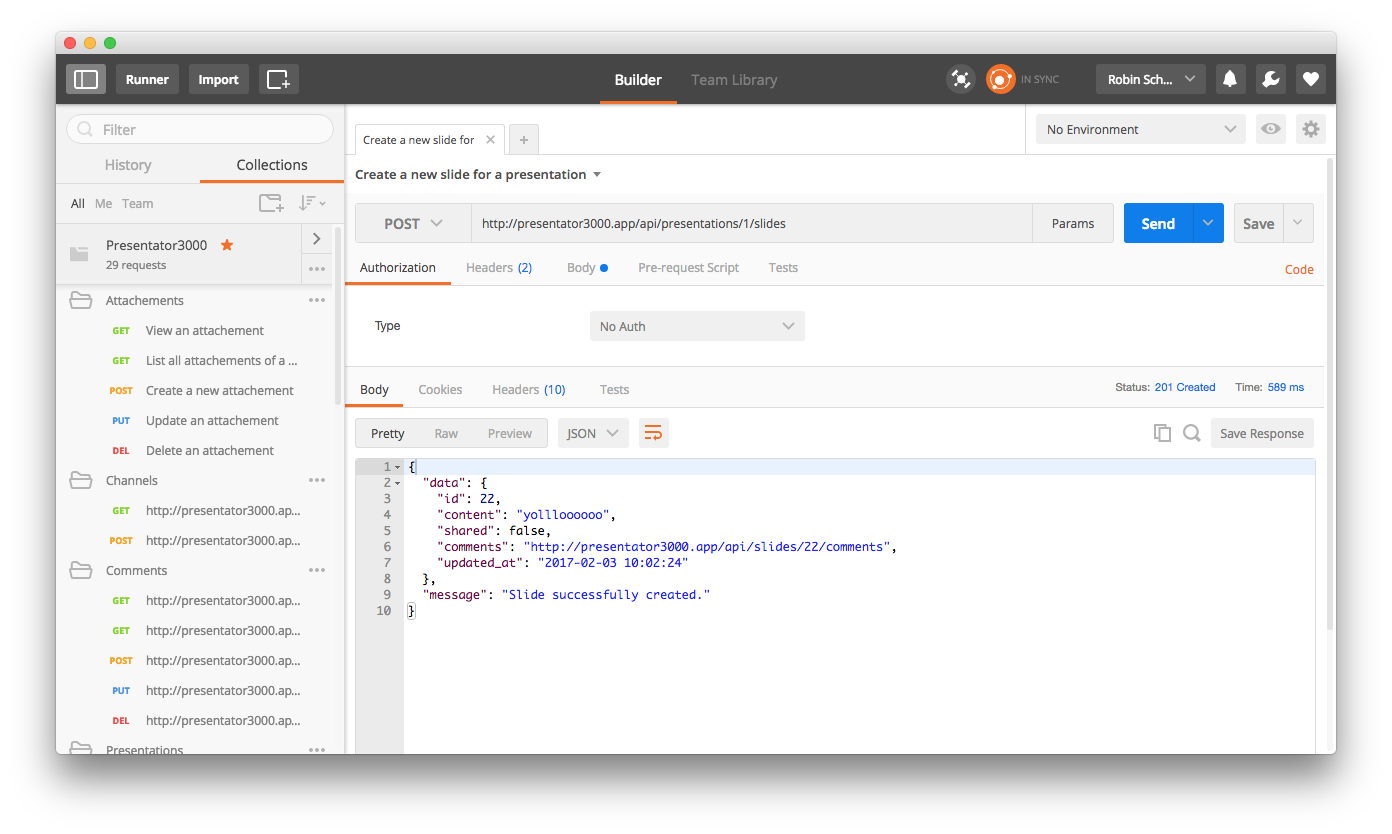
\includegraphics[width=1\textwidth]{images/printscreen-postman.png}
    \caption{Printscreen der Postman Applikation}
\end{figure}